%!TEX root = ../rapport.tex

\chapter{Preliminaries: Basic Lambda Calculus}
\label{chap:theory}

As a very informal example, here is a function that doubles an integer:
\begin{equation*}
	(\lam{x}{x+x})2=4.
\end{equation*}
This example shows a \emph{bound variable}, $x$, and an implicit \emph{reduction step}. The variable $x$
is said to be bound because the lambda function uses it as an argument. Contrast this to
\begin{equation*}
	(\lam{x}{x+y})2=2+y.
\end{equation*}
Here, $y$ is a variable that has no values assigned to it yet. From
the context we can say nothing about $y$, so we give it the predicate
``free''. In this second example there was yet another reduction step, which 
can be regarded as a rewriting action on the string representing the
lambda term. More informally, one can think of it as ``substituting in''
the values for the bound variables. In the examples above this amounts to
replacing $x$ with the number 2.

% definition af syntax
\section{Syntax}
\begin{definition}
	The lambda calculus consists of \emph{lambda terms} defined over the alphabet:
	\begin{align*}
		x,y,z,\hdots\ &\in V\\
		\lambda\ &\text{ abstractor} \\
		()\ &\text{ parentheses}
	\end{align*}
	where $V$ is the countable, infinite set containing variable names $v_0,v_1,v_2,\hdots$.
	The set of all lambda terms $\Lambda$ is defined inductively as follows:
	\label{def:grammar}
	\begin{align*}
		x\in\Lambda \\
		M\in\Lambda &\Rightarrow (\lam{x}{M})\in\Lambda \\
		M, N\in\Lambda &\Rightarrow (M N)\in\Lambda
	\end{align*}
where $x\in V$.
\end{definition}
\begin{convention}
	A term $\lam{x}{M}$ is called a function.
\end{convention}
\begin{convention}
	For brevity, we leave out the outermost parentheses.
\end{convention}
\begin{convention}\label{con:assoc}
	Evaluation is left associative:
	\begin{equation*}
		M N P \equiv (M N) P
	\end{equation*}
\end{convention}
\begin{convention}\label{con:extent}
	Function bodies extend as far as possible:
	\begin{equation*}
		\lam{x}{M N}\equiv\lam{x}{(M N)}\not\equiv(\lam{x}{M})N
	\end{equation*}
\end{convention}
\begin{convention}
	Functions take exactly one argument, but as syntactic sugar we use:
	\begin{equation*}
		\lam{xy}{xy}\equiv\lam{x}{\lam{y}{xy}}
	\end{equation*}
\end{convention}

\section{Free Variables}

As already indicated, the variables in a lambda term can be divided into
two groups; the free and the bound variables.

\begin{definition}
	The set $FV(M)$ is the smallest set containing all free variables of the lambda
	term $M$, defined by:
	\begin{align*}
		FV(x)&=\{x\} \\
		FV(\lam{x}{M})&= FV(M) - \{x\} \\
		FV(M N) &= FV(M) \cup FV(N)
	\end{align*}
\end{definition}
\begin{definition}\mbox{}
	\begin{enumerate}
		\item If $FV(M)=\emptyset$, $M$ is said to be \emph{closed}.
		\item The set of all closed terms is denoted $\Lambda^0$.
	\end{enumerate}
\end{definition}
\begin{definition}
	A variable $x$ that is not free is \emph{bound}.
\end{definition}

\section{Substitution}

It is possible to substitute
values for free variables. These values are not limited to being just new
variables, but can be any lambda term. A substitution is notated:
\begin{align*}
	M[x:=N]
\end{align*}
with the intuitive meaning that all free occurences of $x$ are replaced with 
the term $N$.
\begin{definition}
Substitution is defined as follows (\cite{Barendregt} 2.1.15):
\begin{align*}
	x[x:=N]&\equiv N \\
	y[x:=N]&\equiv y, \text{ if } x \not\equiv y \\
	(\lam{y}{M})[x:=N]&\equiv\lam{y}{(M[x:=N])}, \text{ if } x\not\equiv y \\
	(\lam{x}{M})[x:=N]&\equiv\lam{x}{M} \\
	(M L)[x:=N]&\equiv(M[x:=N])(L[x:=N])
\end{align*}
\end{definition}
Using this definition, the following result can be shown (\cite{Barendregt} p. 28):
\begin{lemma}\label{lem:subst}\mbox{}
	\begin{enumerate}
		\item $M=M'\Rightarrow M[x:=N]=M'[x:=N]$.
		\item $N=N'\Rightarrow M[x:=N]=M[x:=N']$.
		\item $M=M', N=N'\Rightarrow M[x:=N]=M'[x:=N']$.
	\end{enumerate}
\end{lemma}
Lemma \ref{lem:subst} tells us, informally, that the meaning of a a lambda term
is closed under substitution with equals.

\section{Subterms}

A lambda term $M$ is composed of several parts which we call \emph{subterms}.
\begin{definition}\mbox{}
	\begin{enumerate}
		\item $N\subset M$ denotes that $N$ is a subterm of $M$. The set $Sub(M)$ is the 
		smallest set such that all subterms of $M$ are contained in $Sub(M)$:
		\begin{align*}
			Sub(x) &=\{x\} \\
			Sub(\lam{x}{N}) &= Sub(N) \cup \{\lam{x}{N}\} \\
			Sub(M N) &= Sub(M) \cup Sub(N)  \cup \{M N\} %FIXME det ser da underligt ud?
		\end{align*}
		\item A subterm $N$ of $M$ is called \emph{active} if $N L \subset M$ 
		for a term $L$ and \emph{passive} otherwise.
	\end{enumerate}
\end{definition}
\begin{example}\label{exmpl:subterms}
	The term $M\equiv\lam{x}{xy(\lam{z}{y})}$ has the following subterms:
	\begin{itemize}
		\item $\lam{x}{((xy)(\lam{z}{y}))}\subset M$, passive.
		\item $(xy)(\lam{z}{y})\subset M$, passive.
		\item $xy\subset M$, active.
		\item $\lam{z}{y}\subset M$, passive.
		\item $x\subset M$, active.
		\item $y\subset M$, passive.
	\end{itemize}
\end{example}
Note that the subterm $y$ occurs two times in Example \ref{exmpl:subterms}.

\section{$\alpha$-congruence}

The particular name of a bound variable does not affect the function represented 
by a lambda term. Thus, the two terms
\begin{align*}
	\lam{x}{x} \\
	\lam{y}{y}
\end{align*}
denote the same function, namely the identity. This gives rise to a definition of congruence
that is essential in the lambda calculus.
\begin{definition}\mbox{}
	\begin{enumerate}
		\item For a term $M$, \emph{change of bound variables} is defined as a substitution
		of a part of $M$, $\lam{x}{N}$, with $\lam{y}{N[x:=y]}$, i.e. all occurences of $x$
		are replaced with an occurence of $y$. It is a requirement that $y$ does not 
		occur in $N$.
		\item $M$ and $N$ are $\alpha$-congruent, $M\equiv_\alpha N$, if $N$ is the
		resulting term after a finite sequence of changes of bound variables in $M$.
	\end{enumerate}
\end{definition} 
For instance, we have:
\begin{example}
\begin{align*}
	\lam{x}{x}&\equiv_\alpha\lam{y}{y} \\
	\lam{x}{\lam{y}{xy}}&\equiv_\alpha{\lam{a}{\lam{b}{ab}}} \\
	\lam{x}{\lam{y}{xy}}&\not\equiv_\alpha\lam{y}{\lam{y}{yy}}
\end{align*}
\end{example}
This last example illustrates the need for the requirement that $y$ cannot
occur in $N$. 
\begin{convention}
	\label{con:alpha}
	In the following we will regard $\alpha$-congruent terms as
	being equivalent, so the notation $\equiv$ is used instead of
	$\equiv_\alpha$.
\end{convention}

\section{Contexts}

\begin{definition}\mbox{}
	\begin{enumerate}
		\item A context $C[\ ]$ is an ``unfinished term'' with one hole in it. 
		\item The set $Con$ contains all contexts and is defined as the smallest
		set satisfying these constraints:
		\begin{align*}
			[\ ]&\in Con \\
			M\in\Lambda\Rightarrow M[\ ]&\in Con \\
			M\in\Lambda\Rightarrow [\ ]M&\in Con \\
			C\in Con\Rightarrow \lam{x}{C} &\in Con
		\end{align*}
		\item Terms can be plugged into the holes, thus completing the term. 
		\item When plugging a term into a hole, we do not work modulo 
		$\alpha$-congruence.
	\end{enumerate}
\end{definition}
\begin{example}
	Given the context $C[\ ]\equiv\lam{x}{x[\ ]}$, we can make new lambda terms:
	\begin{align*}
		C[x]&\equiv\lam{x}{xx} \\
		C[\lam{y}{y}]&\equiv\lam{x}{x\lam{y}{y}}
	\end{align*}
\end{example}

\section{$\beta$-reduction}

In this section we shall define a key concept of the lambda calculus which
plays a central role in this report, namely the $\beta$-reduction. This
reduction captures the notion of ``substituting in'' terms for bound variables,
and can be intuitively thought of as ``solving'' a lambda term by reducing it
to a (sometimes) simpler form.

\begin{definition}\label{def:betareduction}\mbox{}
	\begin{enumerate}
		\item \emph{$\beta$-reduction} is a binary relation $\BETA\subseteq\Lambda^2$ such that
		\begin{equation*}
			\BETA=\Big\{\big((\lam{x}{M})N,\ M[x:=N]\big)\big|M,N\in\Lambda\Big\}.
		\end{equation*}
		\item For an element $(M,N)\in\BETA$ we call $M$ a \emph{$\beta$-redex} and
		$N$ a \emph{$\beta$-contractum} of $M$.
		\item A term $M$ is in \emph{$\beta$-normal-form} ($\beta$-nf) if it 
		does not contain any subterms that are $\beta$-redexes.
	\end{enumerate}
\end{definition}
\begin{definition}
	Definition \ref{def:betareduction} is extended to contexts.
	\begin{align*}
		C\big[(\lam{x}{M})N\big]\equiv C\big[M[x:=N]\big]
	\end{align*}
\end{definition}
\begin{definition}\label{def:beta_rel1}
	We have the relations (\cite{Barendregt} def. 3.1.5]):
	\begin{align*}
		(M,N)\in\BETA&\Rightarrow M\barrow N \\
		M\barrow N &\Rightarrow ZM\barrow ZN \\
		M\barrow N &\Rightarrow MZ\barrow NZ \\
		M\barrow N &\Rightarrow \lam{x}{M}\barrow \lam{x}{N} 
	\end{align*}	
\end{definition}
\begin{definition}\label{def:beta_rel2}
	The transitive, reflexive closure of $\barrow$ is notated $\Barrow$:
	\begin{align*}
		M\barrow N &\Rightarrow M\Barrow N \\
		M\Barrow N, N\Barrow L &\Rightarrow M\Barrow L \\
		M\Barrow M & 
	\end{align*}
\end{definition}
\begin{definition}
	The relations from Definitions \ref{def:beta_rel1} and \ref{def:beta_rel2} 
	generate an equivalence relation:
	\begin{align*}
		M\Barrow N &\Rightarrow M=_\beta N \\
		M=_\beta N &\Rightarrow N=_\beta M \\
		M=_\beta N\wedge N=_\beta L&\Rightarrow M=_\beta L
	\end{align*}	
\end{definition}
\begin{definition}
	A term $N$ is a \emph{$\beta$-normal form of $M$} if $M=_\beta N$ and $N$ is in $\beta$-normal form.
\end{definition}
\begin{definition}
	For two terms, $M\Barrow N$, we call $N$ the \emph{reduct} of $M$.
\end{definition}
From these definitions it follows (\cite{Barendregt} 3.1.10), that if $M$ is a
$\beta$-nf then $\neg\exists N:M\barrow N$ and $M\Barrow N\Rightarrow M\equiv N$.

The following example from \cite{Barendregt} p. 52 illustrates the concept:
\begin{example}
	$(\lam{x}{xx})(\lam{y}{y})z\Barrow z$, and hence $(\lam{x}{xx})(\lam{y}{y})z =_\beta z$.
	More elaborately:
\begin{align*}
	(\lam{x}{xx})(\lam{y}{y})z&\barrow(\lam{y}{y})(\lam{y}{y})z \\
	&\barrow(\lam{y}{y})z \\
	&\barrow z
\end{align*}
\end{example}

\section{The Church-Rosser Theorem}

A very important property of the lambda calculus was shown by Church and
Rosser \cite{Church1936}. The following formulations are from
\cite{Barendregt} Chapter 3.

\begin{definition}\mbox{}
	\begin{enumerate}
	\item A binary relation $\rightarrow\subseteq\Delta^2$ satisfies the \emph{diamond property}
	($\rightarrow\models\diamondsuit$) if:
	\begin{align*}
		\forall M,M_1,M_2 : \big(M\rightarrow M_1\wedge M\rightarrow M_2
		\Rightarrow \exists M_3 : \left(M_1\rightarrow M_3 \wedge M_2 \rightarrow M_3\right) \big)
	\end{align*}
	
	\item A relation whose reflexive, transitive closure satisfies the diamond property
	is \emph{Church-Rosser} (CR).
	\end{enumerate}
\end{definition}

A look at Figure \ref{fig:images_diamond} explains why it is called the ``diamond property''.

\begin{figure}[htbp]
	\centering
		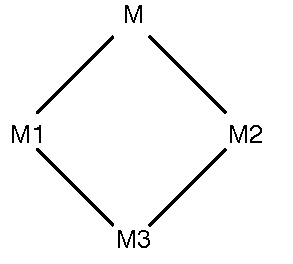
\includegraphics[height=1in]{../images/diamond.pdf}
	\caption[The diamond property.]
	{The diamond property. The lines represent binary relations between the elements.}
	\label{fig:images_diamond}
\end{figure}

\begin{theorem}[Church-Rosser Theorem]\mbox{}
	\begin{enumerate}
		\item The $\beta$-reduction, $\BETA\subseteq\Delta^2$ satisfies the
		diamond property.
		\item The reflexive, transitive closure of the $\beta$-reduction, $\Barrow$, satisfies
		the diamond property. Hence, the $\beta$-reduction is Church-Rosser.
	\end{enumerate}
\end{theorem}

The Church-Rosser theorem implies, informally, that a $\beta$-reduction cannot
get ``stuck'', unless a normal form is being reduced.

\section{Reduction Graphs}

When a $\beta$-redex $M$ contains subterms $\Delta_{0\hdots n}$ that are themselves 
$\beta$-redexes, an ambiguity concerning the order of $\beta$-reductions arises.
Consider the following example from \cite{Barendregt} 3.1.19:
\begin{example}
	Let $M\equiv(\lam{x}{xx})\Delta$ and $\Delta\barrow\Delta'$. We can then perform the two reductions:
\begin{align*}
	M&\barrow(\lam{x}{xx})\Delta' \\
	M&\barrow\Delta\Delta
\end{align*}
\end{example}
The example shows that we can choose to reduce $\Delta$ to its contractum $\Delta'$, or
we can choose to reduce $M$ to its contractum $\Delta\Delta$. This is notated as 
$\overset{\Delta}\barrow$ and $\overset{M}\barrow$ respectively. Different
subterms can have the same contractum, as this example illustrates:
\begin{example}
	Let $\I\equiv\lam{x}{x}$. Then:
\begin{align*}
	\I(\I x)&\overset{\I x}\barrow\I x \\
	\I(\I x)&\overset{\I(\I x)}\barrow\I x
\end{align*}
\end{example}
The set of reductions from a redex $M$ can
be considered as a directed graph, with each arc going out of a node representing
a reduction on some subterm of that node, and each node representing a lambda term that
is the contractum of the terms represented by the nodes parents.
\begin{definition}
	The \emph{$\beta$-reduction graph} of $M$, written $G_\beta(M)$, consists
	of the nodes in the set $V$ and the arcs in the multiset $A$. The set
	of nodes and multiset of arcs in $G_\beta(M)$ are defined as:
	\begin{align*}
		V&=\{N\in\Lambda|M\Barrow N\} \\
		A&=\{(N_0, N_1)\in\Lambda^2|N_0,N_1\in V\wedge N_0\barrow N_1\}
	\end{align*}
	Since $A$ can contain duplicates it follows that if there are more than one
	different reduction step from $N_0$ to $N_1$, that many arcs will be included 
	in $G_\beta(M)$.
\end{definition}

\begin{example}\mbox{}
	\begin{enumerate}
		\item The reduction graph illustrated in Figure \ref{fig:images_graphs_graf2}
		for the term $\I x$, $G_\beta(\I x)$, with
		the previous definition of $\I$ captures the reduction $\I x\barrow x$.
		
		\item $G_\beta(\I(\I x))$ is illustrated in Figure \ref{fig:images_graphs_graf1}.
		
		\item Let $\Omega\equiv(\lam{x}{xx})(\lam{x}{xx})$. $G_\beta(\Omega)$
		can be seen in Figure \ref{fig:images_graphs_graf3_omega}.
		
		\item Let $\W\equiv\lam{xy}{xyy}$. $G_\beta(\W\W\W)$ is illustrated in
		Figure \ref{fig:images_graphs_graf4_www}.
		
		\item Let $M\equiv\lam{x}{(\lam{y}{yy})x}$. $G_\beta(MM)$ is pictured in
		Figure \ref{fig:images_graphs_graf5_MM}.
		
		\item Let $w_3\equiv\lam{x}{xxx}$. Figure \ref{fig:images_graphs_graf6_w3w3}
		contains the reduction graph. Note that this graph contains an infinite 
		amount of nodes and arcs.
		
		\item In Figure \ref{fig:images_graphs_graf7_omega_w3} there is another
		example of a graph containing an infinite amount of nodes and arcs. This
		graph captures qualities found in the two graphs $G_\beta(\Omega)$ and
		$G_\beta(w_3w_3)$.
	\end{enumerate}
	Note that these examples only serve to illustrate the \emph{structure} of a 
	$\beta$-reduction graph, not the actual graph visualization that we develop
	in this paper.
	\begin{figure}[htbp]
		\centering
		\begin{tabular}{ccc}
			\subfigure[$G_\beta(\I x)$]{
				
\includegraphics{../images/graphs/graf2.pdf}
				\label{fig:images_graphs_graf2}
			} &
			\subfigure[$G_\beta(\I(\I x))$]{
				
\includegraphics{../images/graphs/graf1.pdf}
				\label{fig:images_graphs_graf1}
			} & 
			\subfigure[$G_\beta(\Omega)$]{
				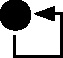
\includegraphics{../images/graphs/graf3_omega.pdf}
				\label{fig:images_graphs_graf3_omega}
			} \\ \\
			\subfigure[$G_\beta(\W\W\W)$]{
				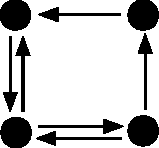
\includegraphics{../images/graphs/graf4_www.pdf}
				\label{fig:images_graphs_graf4_www}
			} \hspace{1.5em}
			&
			\subfigure[$G_\beta(MM)$]{
				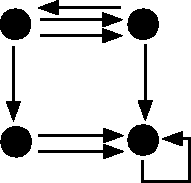
\includegraphics{../images/graphs/graf5_MM.pdf}
				\label{fig:images_graphs_graf5_MM}
			}\hspace{1.5em}
			&
			\subfigure[$G_\beta(w_3w_3)$]{
				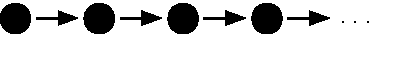
\includegraphics{../images/graphs/graf6_w3w3.pdf}
				\label{fig:images_graphs_graf6_w3w3}
			}
		\end{tabular}
		\caption
		[Examples of $\beta$-reduction graphs for different lambda terms.]
		{Examples of $\beta$-reduction graphs for different lambda terms. 
		Taken from \cite{Barendregt}.}
	\end{figure}
	\begin{figure}[htbp]
		\centering
			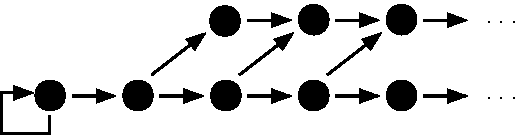
\includegraphics{../images/graphs/graf7_omega_w3.pdf}
		\caption{The $\beta$-reduction graph $G_\beta(\Omega w_3)$}
		\label{fig:images_graphs_graf7_omega_w3}
	\end{figure}
\end{example}

Not all directed graphs are reduction graphs. Because of the Church-Rosser
property, reduction graphs like the ones pictured in Figure
\ref{fig:images_graphs_impossible} cannot exist for any lambda term. Any graph
with more than two nodes with an in-degree of 1 cannot be a reduction graph in
the lambda calculus because of this property. In \cite{VenturiniZilli1984251}
are more thorough discussion of what cannot be a reduction graph is presentd.

\begin{figure}[htbp]
	\centering
	\subfigure[The diamond property is obviously violated in this graph.]{
		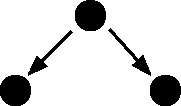
\includegraphics{../images/graphs/impossible1.pdf}
	}
	\subfigure[It is too in this graph; no less than three normal forms
	should be produced in order to make this graph.]{
		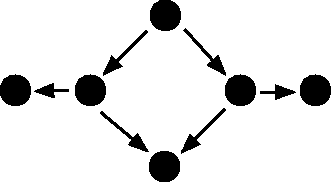
\includegraphics{../images/graphs/impossible2.pdf}
	}
	
	\caption{Examples of directed graphs that cannot be reduction graphs.}
	\label{fig:images_graphs_impossible}
\end{figure}
